\documentclass[conference]{IEEEtran}

\usepackage{listings}
\usepackage{pgfplots}
\pgfplotsset{compat=1.6}
\usepackage{hyperref}
\usepackage{caption}
\usepackage{subcaption}
\usepackage{tikz}

\usepackage[
  backend=biber,
  style=ieee,
  sorting=none
]{biblatex}
\addbibresource{CAD.bib}

\lstset{basicstyle=\footnotesize\ttfamily,
  breaklines=true}




\begin{document}

\title{Performance enhancement using MPI in a simulation of heat diffusion}

\author{
  \IEEEauthorblockN{Gonçalo Lourenço \\ nº55780 \\ gm.lourenco@campus.fct.unl.pt}
  \and
  \IEEEauthorblockN{Joana Faria \\ nº55754 \\ js.faria@campus.fct.unl.pt}
}

\maketitle



\section{Introduction}
This assignment aims to optimize a base code, written in \texttt{C}, that computes a simulation for heat diffusion. This time we intend to parallelize the computation using the Message Passing Interface (MPI).

To find the best performance we will explore different approaches, namely analyzing different patterns of communication and trying to overlap the communication with the computation.

We have available, for this assignment, two nodes, each one with 16 true CPUs.\@ Given this information, we can have a maximum of 32 processes.


\section{Results}
We experiment with many versions of a parallel program using MPI, these versions are explained and analyzed below.

To establish a baseline for comparison we start by analyzing the execution time of the sequential version and we obtain an average of 153.979 seconds, with the following parameters:
\begin{verbatim}
  // Width of the area
  const int nx = 200;
  // Height of the area
  const int ny = 200;
  // Diffusion constant           
  const float a = 0.5;
  // h=dx=dy  grid spacing
  const float h = 0.005;
  // Number of time steps to simulate
  const int numSteps = 100000;  
  // How frequently to write output image
  const int outputEvery = 100000;
\end{verbatim}

Unless otherwise stated, these will be the parameters used for determining the execution times.

\section{Discussion}

\subsection{V1 version --- Synchronous Communication}\label{sec:v1}

In version V1 we start with a simple parallel version where we distribute the lines of the original matrix by the number of processes and perform synchronous communication between neighbors processes to obtain the border necessary for the computation.

For the communication necessary to write the output we use the \texttt{MPI\_Send} and \texttt{MPI\_Recv} methods, where all process sends their results to process 0, which aggregates all the results and writes the output file.

In \autoref{fig:executionTimeV1} we can see the execution time for V1, comparing the performance of this version for different numbers of processes.

\begin{figure}[ht]
  \centering
  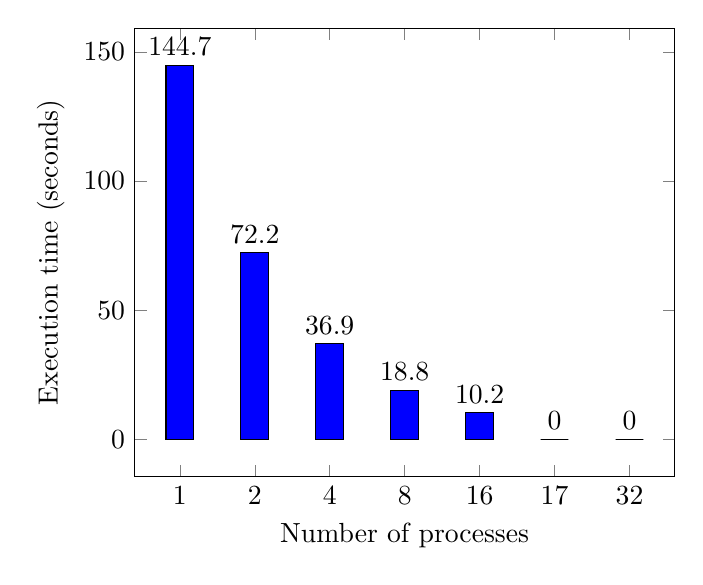
\begin{tikzpicture}

    \begin{axis}[
        ylabel={Execution time (seconds)},
        xlabel={Number of processes},
        symbolic x coords={1,2, 4, 8, 16, 17, 32},
        xtick=data,
        nodes near coords={
            \pgfmathprintnumber[precision=1]{\pgfplotspointmeta}
          },
      ]
      \addplot[ybar,fill=blue] coordinates {
          (1,   144.74)
          (2,   72.22)
          (4,  36.92)
          (8,   18.83)
          (16,   10.23)
          (17,   0)
          (32,   0)
        };
    \end{axis}
  \end{tikzpicture}
  \caption{Execution time of V1 varying the number of processes}
  \label{fig:executionTimeV1}
\end{figure}

\subsection{V2 --- Gather}\label{sec:v2}
In this version, we modify version V1 to use the method \texttt{MPI\_Gather} for the phase of writing the output.




\section{Compilation and Execution Instructions}
Our best version, V2, can be compiled and executed with the following command, from inside the folder \texttt{/proj1}:
\begin{verbatim}
nvcc -o v2 v2.cu && ./v2
\end{verbatim}
This will execute ten iterations to measure the average execution times and the results of the heat equation will be saved in the folder \texttt{images/v2}.


\printbibliography


\end{document}